\entry{Semana del 29/09/2025.} 

\section{Lunes 29/09/2025.} 
Esta semana me toca dar a mí la Reunión del grupo, así que probablemente vaya a estar dedicándome esencialmente a eso. En otras noticias: 

\begin{itemize}
	\item Ya estaban impresas (desde el Viernes pasado) y fui a buscar las carcasas para los dos nuevos sensores (tenemos ya 4 en total), que vinieron casi todas de nuevo con sus soportes de impresión. Faltaría montarlos pero no creo que vaya a ser hoy. 
	\item Ya compró Pablo y recibió el cable bipolar para la conexión de los sensores, faltarían las puntas de cocodrilo. El cable es bastante finito, por ahí sea necesario agregar soldadura a las puntas, pero no creo que moleste mucho más que para eso. 
\end{itemize} 

\subsection*{Funciones de estructura de más puntos.} 
En vistas de la charla me puse a hacer un par de cosas que habían quedado pendientes. En primer lugar calcular las funciones de estructuras y PDFs de las $\Delta \eta(\tau)$, como lo de la semana del 25/08/2025, usando diferencias de más puntos. Acá abajo para las diferencias de 4 puntos, definidas en \cite{angrimanMultitimeStructureFunctions2022}: 

\begin{equation}
	\Delta\eta(\tau) = \eta(t+\eta) - 3\eta(t) + 3\eta(t-\tau) - \eta(t-2\tau)
\end{equation}

En primer lugar las PDFs que dieron bastantes parecidas. 

\begin{figure}[!ht]
	\centering
	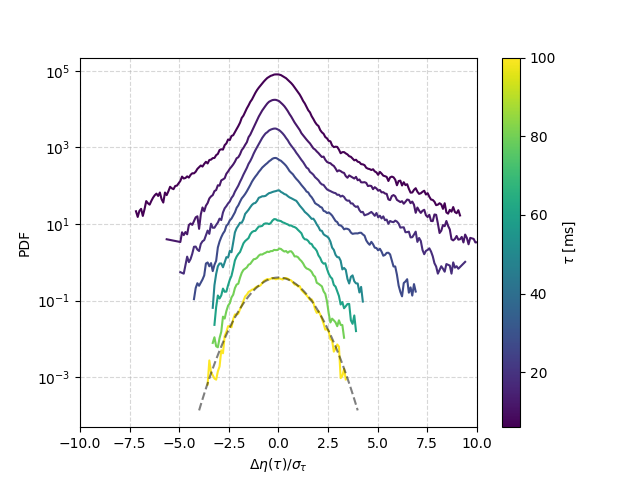
\includegraphics[width=0.7\linewidth]{Figures/29_09_2025/PDFs_deltas_para_4pt_0_6Hz}
	\caption{PDFs de las $\Delta\eta(\tau)$ para diferencias de 4 puntos en la medición de 0-6 Hz.}
	\label{fig:pdfsdeltaspara4pt06hz}
\end{figure}

Y después las funciones de estructura en sí. Da en general también bastante parecido, pero se aplana el rebote del final.  

\begin{figure}[th!]
	\centering
	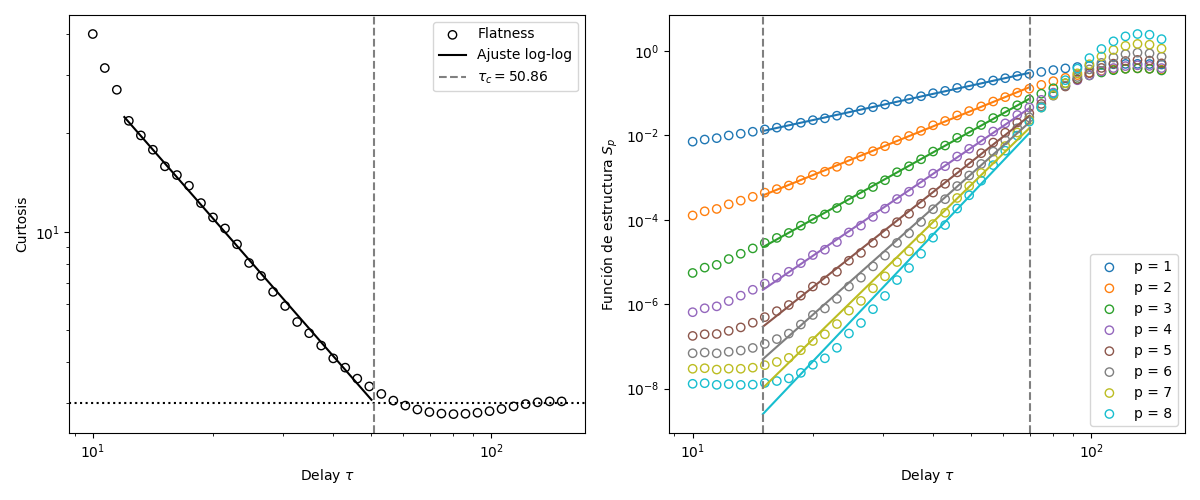
\includegraphics[width=0.879\linewidth]{Figures/29_09_2025/SP_deltas_4pt_0_6Hz}
	\caption{Flatness y funciones de estructura para las diferencias de 4 puntos en la banda de 0-6 Hz. La pendiente de la curtosis dió -1.392 y el tiempo de correlación de 50.857 ms.} % : 
	\label{fig:spdeltas4pt06hz}
\end{figure}

Por último la evolución de los exponentes. % : 

\begin{figure}[th!]
	\centering
	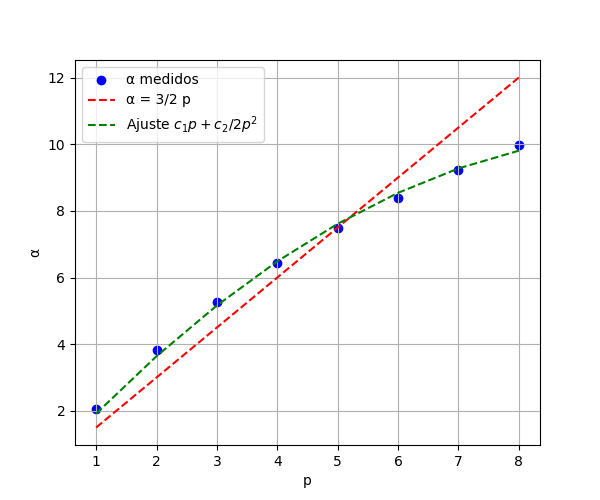
\includegraphics[width=0.587\linewidth]{Figures/29_09_2025/Exponentes_SP_deltas_4pt_0_6Hz}
	\caption{Exponentes de las funciones de estructura en función del orden para la banda de 0-6 Hz usando las diferencias de 4 puntos.}
	\label{fig:exponentesspdeltas4pt06hz}
\end{figure}

Acá no estoy seguro de la pendiente teórica, probablemente habría que estimar una nueva usando análisis dimensional (está puesta la de tres puntos). Faltaría además ponerle los errores a esos puntos (en este gráfico y en los anteriores).  

Probé usar la velocidad $v=\frac{d\eta}{dt}$ en vez usar $\eta$ pero dan todas las PDFs básicamente Gaussianas. 


\section{Viernes 03/10/2025.} 

Hoy fue la charla en la reunión de grupo. En general estoy bastante conforme con como salió y surgieron varias preguntas y discusiones interesantes de las que dejo constancia acá abajo: 

\begin{itemize} 
	\item Sobre la introducción: 
	\begin{itemize} 
		\item Para qué sirve exactamente la aproximación  de fase aleatoria. No es necesaria para llegar a la evolución de las amplitudes de onda pero sí para clausurar la jerarquía de ecuaciones al buscar la evolución temporal de la acción de ondas $n(\vec k)$. 
	\end{itemize}
	\item Sobre el sensor capacitivo: 
	\begin{itemize}
		\item Sobre cómo es la distribución de errores del sensor, si resulta simétrica. 
		\item Existe un spray hidrofóbico que podríamos usar para recubrir el alambre y ver si los $\pm0.1$ mm salen de ahí. 
		\item La frecuencia de corte máxima que puede resolver el motor debería ser aquella que se corresponda con el diámetro del mismo (creo que ra del orden de $6$ kHz). 
		\item Ver además de qué orden de frecuencia es el 0.1 mm. 
	\end{itemize} 
	\item Sobre la experiencia de turbulencia de ondas: 
	\begin{itemize}		
		\item si usamos 5 cm de agua destilada y las ondas tienen 1 cm de amplitud porqué sería válido seguir pensando en la aproximación de profundidad infinita. En general funciona bien y es lo que suele usar la gente en otros experimentos similares. 
		\item ¿Sería necesario agregar obstáculos que rompan los modos normales de la caja? En principio tienen frecuencias bajas así que no deberían molestar demasiado. 
	\end{itemize}	
	\item Sobre los primeros resultados: 
	\begin{itemize}
		\item Sobre porqué al aumentar la no linealidad se van volviendo asimétricas las PDFs. Si tenía algo que ver con la profundidad finita, pero también aparece en océano.  
		\item En los espectros calcular los exponentes usando las PDFs de las derivadas logarítmicas y luego estimar con el espectro compensado o las misma derivada en qué rangos de frecuencia vale cada régimen y su cruce. 
		\item Estimar el tiempo no lineal para saber si es lo suficientemente alto como para pasarnos del punto en que el espectro da muy bien al momento en que se empieza a romper. 
	\end{itemize}
	\item Sobre los resultados de las interacciones a $N$ ondas: % .
	\begin{itemize}
		\item En el plot 3D para $C(f_1, f_2, f_3)$ se ven dos rectas muy marcadas que son las de $45^\circ$ cuando alguna frecuencia da 0, que son las soluciones triviales cuando $f_2=0$ o $f_3=0$ y entiendo que la tercera de $f_1=0$ no. 
		\item Esa misma correlación se podría calcular en el espacio real con el tiempo agregando delays. 
		\item ¿Sería correlación entre amplitudes o fases? Porque las fases son aleatorias, pero lo que nos importa es lo que pasa con el término de $\omega t$ en esas fases. 
		\item Porqué hay interacciones de tres ondas en gravedad.  	
		\item Probar a calcular las correlaciones sin normalizar y ver si la amplitud decrece según la población de los distintos modos en el espectro. 
		\item Se podría intentar ir a Shallow o alguna altura que haga que gravedad sea shallow (tipo la longitud capilar).  
	\end{itemize}
	\item Sobre los resultados de intermitencia: 
	\begin{itemize}
		\item Para las funciones de estructura en sí, habría que estimar de alguna forma si el cálculo hasta orden 8 está justificado, si podríamos calcular más o menos en función de nuestra cantidad de puntos. % x 
		\item Al tener dos regímenes habría que revisar para cual es el estimado dimensional de los exponentes, pero en principio debería ser para el de capilar por los $\tau$'s en que vale. 
		\item Para la función con las que ajustamos los exponentes $\zeta_p=c_1p-\frac{c_2}{2}p^2$ hay que tener cuidado de no llamarlo modeo ya que en principio va a tener un máximo, y esperaríamos que los exponentes crezcan monótonamente. Además en algún punto se van a volver negativos.  
	\end{itemize} 
\end{itemize}

Además terminé de ensamblar los dos nuevos sensores, aunque faltaría esmaltarlos.  

